% %\documentclass[oneside,final,14pt]{article}
\documentclass[14pt,oneside,final]{extreport}
\usepackage[utf8]{inputenc} 
\usepackage[english,russian]{babel}

\usepackage{vmargin}
\setpapersize{A4}
\setmarginsrb{20mm}{20mm}{20mm}{20mm}{0pt}{0mm}{0pt}{13mm}
\usepackage{indentfirst}
\usepackage{pscyr} % Нормальные шрифты
\DeclareUnicodeCharacter{00A0}{~}
\usepackage[T2A]{fontenc} % Поддержка русских букв
\usepackage{url}
\usepackage{tabularx}
\usepackage{amsmath}
\usepackage{pdfpages}
\usepackage{tikz}

\newcolumntype{Z}{>{\centering\let\newline\\\arraybackslash\hspace{0pt}}X} %новый тип столбца для таблицы

\newcommand*\minus{\item[--]} %для списков

\usepackage[nooneline]{caption} 
\captionsetup[table]{justification=raggedleft} 
\captionsetup[figure]{justification=centering,labelsep=endash} 

\usepackage{titlesec}

\usepackage{subcaption}

\titleformat{\chapter}[display]
{\normalfont\centering\bfseries}
{\MakeUppercase{\chaptertitlename} \thechapter}
{0pt}
{\MakeUppercase}
[]
     
\titleformat{\section}
{\normalsize\bfseries}
{\thesection}
{1em}{}
     
\titleformat{\subsection}
{\normalsize}
{\thesubsection}
{1em}{}
     
% Настройка вертикальных и горизонтальных отступов
\titlespacing*{\chapter}{0pt}{-30pt}{8pt}
\titlespacing*{\section}{\parindent}{*4}{*4}
\titlespacing*{\subsection}{\parindent}{*2}{*2}
    
% всавка изображений
%\ifx\pdfoutput\undefined
%\usepackage{graphicx}
%\else
%\usepackage[pdftex]{graphicx}
%\fi
% сквозная нумерация
\usepackage{chngcntr}
\counterwithout{figure}{chapter}
% сквозная нумерация формул
\renewcommand{\theequation}{\arabic{equation}}

\renewcommand{\thefigure}{\arabic{figure}}
\usepackage[tableposition=top]{caption}
\usepackage{subcaption}
\DeclareCaptionLabelFormat{gostfigure}{Рисунок #2}
\DeclareCaptionLabelFormat{gosttable}{Таблица #2}
\DeclareCaptionLabelSeparator{gost}{~---~}
\captionsetup{labelsep=gost}
\captionsetup[figure]{labelformat=gostfigure}
\captionsetup[table]{labelformat=gosttable}
\captionsetup{figurewithin=none, tablewithin=none} %сквозная нумерация таблиц
\renewcommand{\thesubfigure}{\asbuk{subfigure}}

\linespread{1.3}
\usepackage[toc,page]{appendix}
    \renewcommand\appendixname{Приложение}
    \makeatletter
    \def\redeflsection{\def\l@section{\@dottedtocline{1}{1.5em}{7.8em}}}
    \renewcommand\appendix{\par
    \setcounter{section}{0}%
    \setcounter{subsection}{0}%
    \def\@chapapp{\appendixname}%
    \addtocontents{toc}{\protect\redeflsection}
    \def\thesection{\appendixname\hspace{0.2cm}\@arabic\c@section}}
    \makeatother


\sloppy


\begin{document}
	
	\setboolean{@twoside}{false}
	\includepdf[pages=-,offset=73 -75,pagecommand={
		\clearpage
		\thispagestyle{empty}
		\begin{tikzpicture}[remember picture, overlay]
			\node at (9, -4.9) {Робототехника и комплексная автоматизация};
			\node at (9, -5.8) {Компьютерные системы автоматизации производства};
			\node at (9, -11.45) {Интегрированная система поддержки принятия решения о выборе};
			\node at (9, -12.3) {режимов механической обработки тонкостенных деталей};
			\node at (15.2, -14.45) {П.А. Еремейкин};
			\node at (15.2, -16.25) {А.Д. Жаргалова};
			\node at (15.2, -21.58) {Л.А. Силаева};
			\node at (15.2, -22.88) {А.С. Козодаев};
			\node at (8.37, -25.2) {\small{16}};
		\end{tikzpicture}}]{titul.pdf}
 
	
	\renewcommand*\contentsname{\hfill Содержание \hfill}
	\tableofcontents
	
	
	\chapter{Введение}
	Эксплуатационные характеристики изделий машиностроения в большой мере зависят от качества изготовления деталей, составляющих изделие. Качество изготовления определяется степенью соответствия параметров готовой детали и параметров, достижение которых требуется документацией. В роли такого параметра может выступать точность изготовления геометрических размеров, определяемая допуском. 
	
	Погрешности различных видов препятствуют абсолютно точному воспроизведению заданных параметров. Например, на точность изготовления деталей влияют погрешности базирования, измерения, настройки инструмента и т.д. При обработке нежестких деталей на первый план выходят погрешности, связанные с деформацией самой детали.
	
	Рассмотрим пример обработки тонкостенной детали в трехкулачковом патроне токарного станка. Схема обработки изображена на рисунке~\ref{fig:scheme}. Цифровыми сносками обозначены: 1~-~кулачок патрона, 2~-~цилиндрическая заготовка, 3~-~токарный резец. До начала обработки деталь находится в недеформированном состоянии (рисунок~\ref{fig:scheme-a}). После закрепления детали силы, действующие со стороны кулачков, деформируют заготовку таким образом, что профиль заготовки отличается от идеально цилиндрического (рисунок~\ref{fig:scheme-b}). Дополнительно заготовка деформируется под действием силы резания, а также в связи с нагревом. В процессе резания инструмент неравномерно снимает припуск по окружности заготовки (рисунок~\ref{fig:scheme-c}). После окончания обработки и снятия усилий закрепления отклонение от круглости заготовки достигает величин, сравнимых с величиной допуска и в зависимости от конкретных условий может превышать его (рисунок~\ref{fig:scheme-d}).
	
	\begin{figure*}[t!]
	    \centering
	    \begin{subfigure}[t]{0.5\textwidth}
	        \centering
        	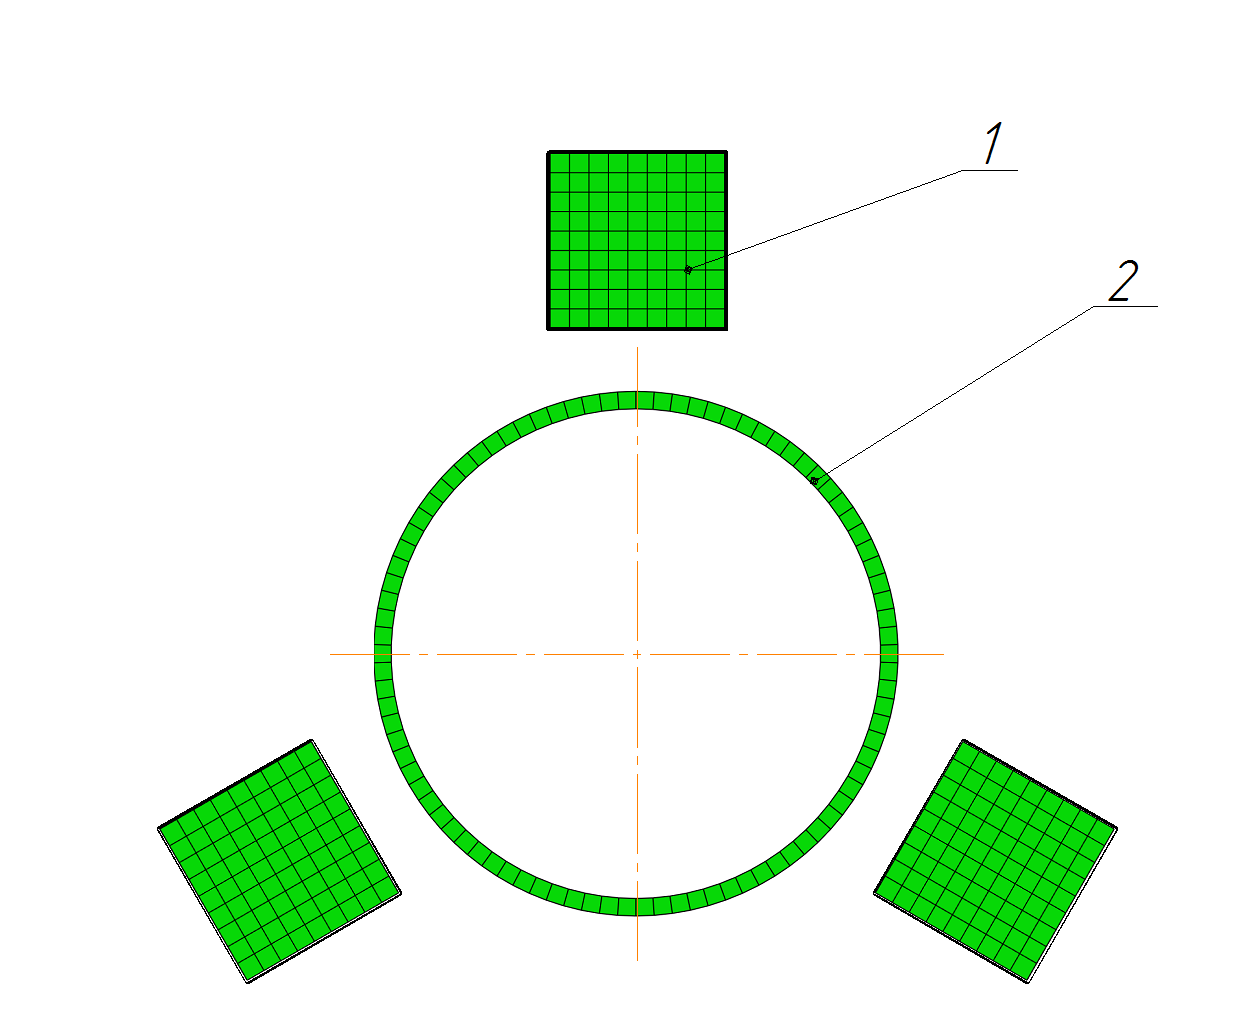
\includegraphics[scale=0.25]{img/scheme-a}
	        \caption{До закрепления} \label{fig:scheme-a}
	    \end{subfigure}%
	    ~ 
	    \begin{subfigure}[t]{0.5\textwidth}
	        \centering
        	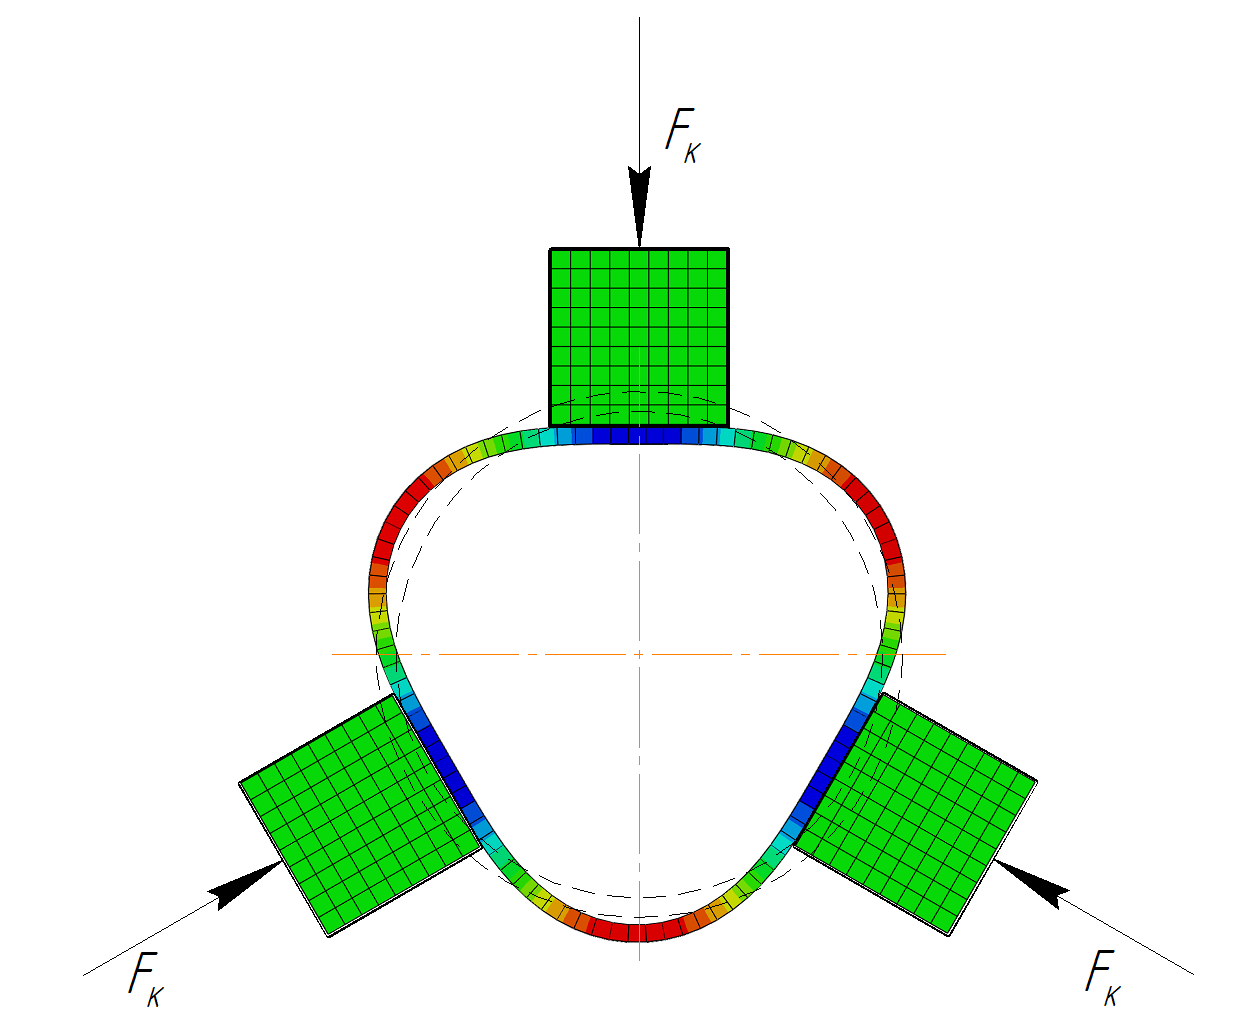
\includegraphics[scale=0.25]{img/scheme-b}
        	\caption{Закрепленная заготовка} \label{fig:scheme-b}
	    \end{subfigure}
	    
   	    \begin{subfigure}[t]{0.5\textwidth}
   	        \centering
           	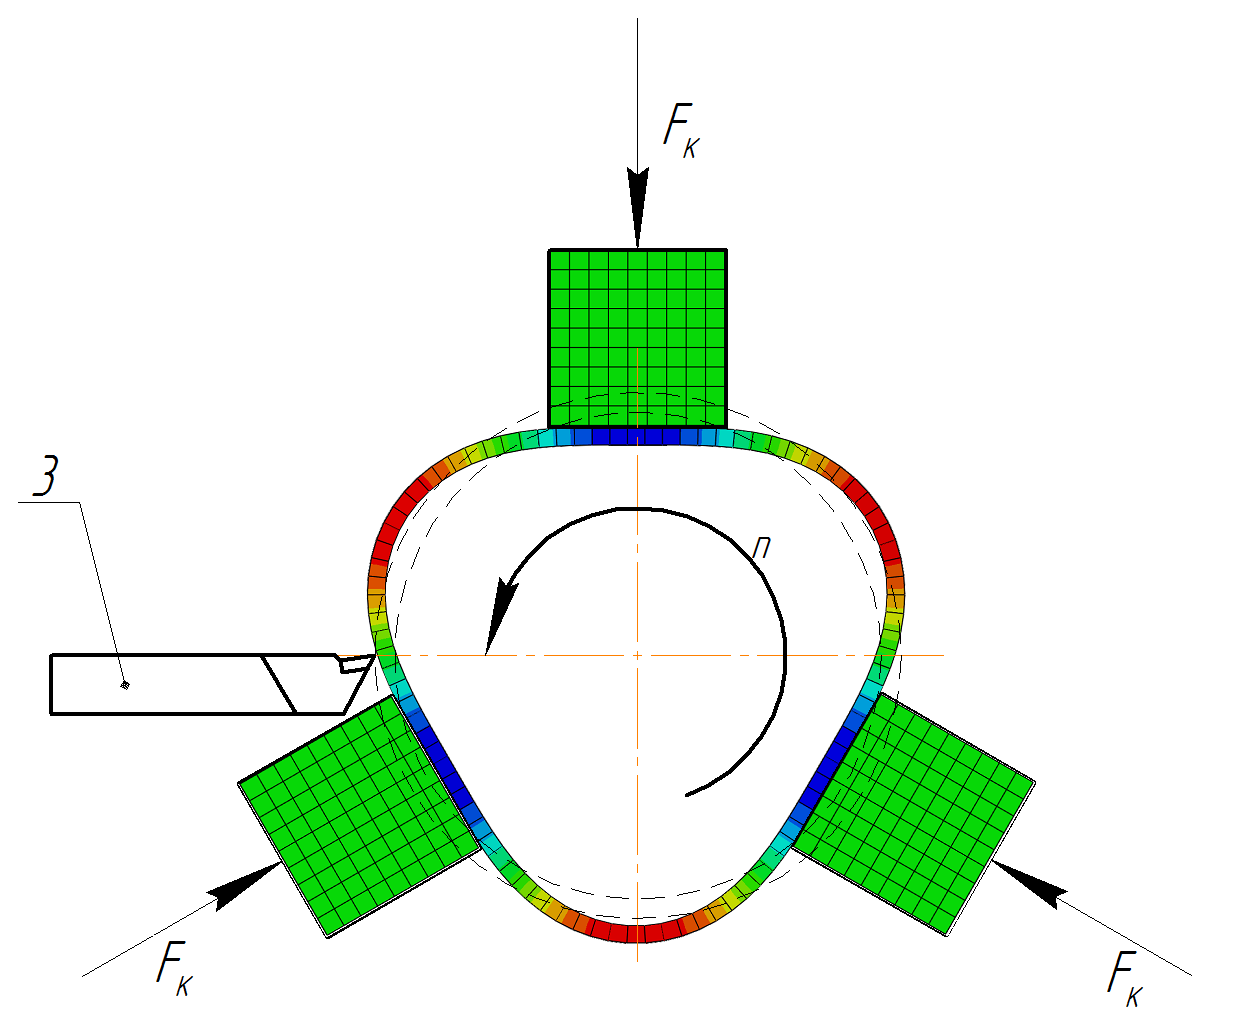
\includegraphics[scale=0.25]{img/scheme-c}
           	\caption{Обработка} \label{fig:scheme-c}
   	    \end{subfigure}%
   	    ~
   	    \begin{subfigure}[t]{0.5\textwidth}
   	       	\centering
   	        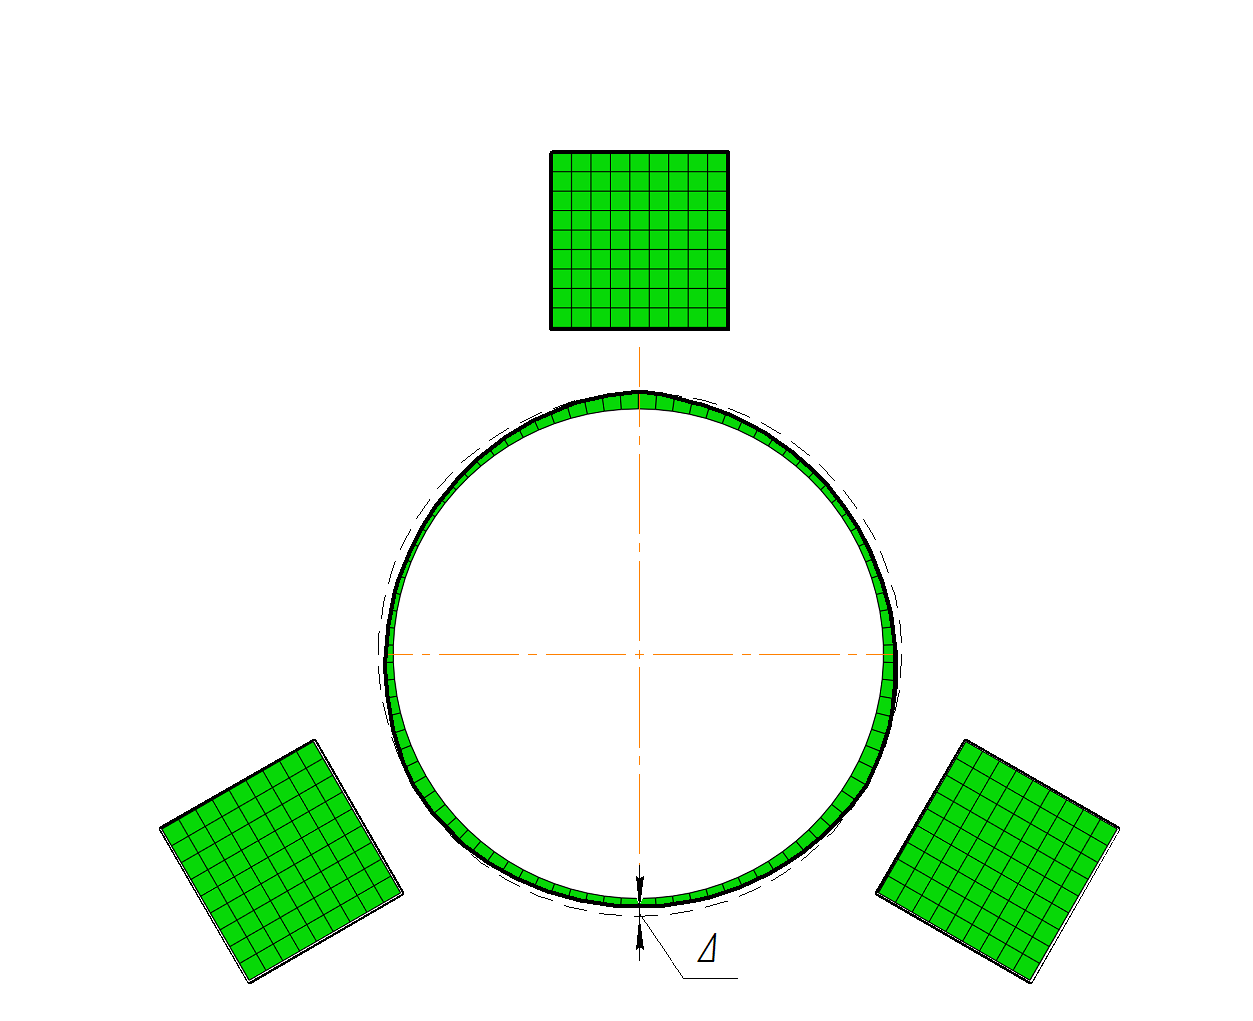
\includegraphics[scale=0.25]{img/scheme-d}
   	    	\caption{Результат} \label{fig:scheme-d}
	   	\end{subfigure}
	    \caption{Обработка тонкостенной заготовки} \label{fig:scheme}
	\end{figure*}


	На практике в случае обработки нежестких деталей применяется специальное технологическое оборудование, позволяющее уменьшить возникающие деформации. Использование сырых кулачков, растрачиваемых под диаметр заготовки - один из способов уменьшения деформаций закрепления. После растачивания кулачок охватывает деталь по большей площади. Также используется обработка с технологическим заполнителем (например, легкоплавким материалом), который увеличивает жесткость детали на время обработки и выплавляется после окончания обработки. Вариант обработки на нормативных режимах резания в специальных приспособлениях привлекателен тем, что он позволяет применять апробированные технологические процессы. Однако, необходимость создания при этом специальных приспособлений требует значительных материальных, производственных и временных затрат. Это удорожает технологическую подготовку производства и увеличивает её сроки. 

	Ввиду указанных ограничений на существующие способы обработки, предлагается рассмотреть еще один метод - подбор режимов обработки и условий закрепления таким образом, чтобы обеспечить изготовление размеров в рамках допуска. Предполагается, что такой метод может найти применение прежде всего в единичном и мелкосерийном производстве, располагающим, как правило, только универсальным оборудованием. Суть подхода заключается в том, чтобы заранее, на этапе разработки технологической документации, определить режимы резания, менее эффективные с точки зрения производительности, но оптимальные с точки зрения точности изготовления. С уменьшением сил резания уменьшаются и деформации заготовки, а также требуемые усилия закрепления, но с другой стороны, увеличивается время обработки.  Подобрав баланс между скоростью и точностью обработки, технолог имеет возможность назначить режимы резания, приемлемые для изготовления заданной детали без привлечения дополнительной технологической оснастки.  Достоинством такого подхода является меньшая ресурсоёмкость и продолжительность технологической подготовки производства. Однако, данный подход в настоящее время ещё не получил достаточного научного обоснования и, как следствие, не поддержан методическими рекомендациями, необходимыми для его применения в промышленных масштабах \cite{article:zhargalova}.
	
	Для поддержки решения о назначении режимов резания предлагается разработать информационную систему, позволяющую анализировать деформации заготовки при заданных геометрических параметрах и режимах резания. Такой инструмент можно использовать для последовательной проверки ряда значений параметров процесса и выбора наиболее рациональных. 
	
	Система, спроектированная в соответствии с современными тенденциями в разработке ПО станет эффективным инструментом для назначения режимов обработки. Объектно-ориентированная модульная архитектура такой системы позволит расширять её функционал в случае возникновения новых требований к применению программы, а независимость от конкретной операционной системы позволит легко внедрить такие системы в процесс разработки технологической документации на предприятиях безотносительно конкретной существующей информационной среды.
	
	
	\chapter{Техническое задание}	
	
	\section{Основания для разработки}
	Основанием для разработки системы являются документы:
	\begin{enumerate}
	\item Задание на выполнение дипломного проекта
	\item Календарный план на выполнение дипломного проекта
	\end{enumerate}
	
	\section{Назначение разработки}
	Функциональным назначением разработки является обеспечение интегрированной рабочей среды для гибкого моделирования процессов деформирования тонкостенных заготовок в процессе их токарной обработки. Под гибкостью понимается возможность изменения параметров процесса в зависимости от расчетного случая и конфигурации заготовки. Эксплуатационным назначением является обеспечение инструментального средства для последовательного определения рациональных режимов резания тонкостенных заготовок и автоматизация сопутствующих расчетов.
	
	\section{Требования к функциональным характеристикам}
	    Система информационной поддержки должна обеспечивать выполнение следующих функций:
	\begin{enumerate}
	\item Расчет деформаций тонкостенной заготовки при токарной обработке с закреплением в кулачковом патроне.
	\item 	Автоматизация необходимых сопутствующих расчетов (режимов резания)
	\item 	Изменение параметров рассматриваемого процесса: геометрии заготовки  и оснастки и значений силовых факторов (силы резания и закрепления)
	\item 	Представление результатов расчета в виде графиков или таблиц деформаций
	\item 	Генерация отчета по результатам расчета
	\item 	Вывод дополнительных информационных отладочных сообщений 
	\end{enumerate}

	\section{Требования к надежности}
	Разрабатываемая система должна обеспечивать надежную работу в условиях ошибочного пользовательского ввода. При возникновении системных исключительных ситуаций необходимо обеспечить их обработку чтобы не допустить аварийного завершения программы.

	\section{Условия эксплуатации}
	Аппаратные   средства   должны   эксплуатироваться   в помещениях с выделенной розеточной электросетью 220В \(\pm\) 10\%, 50 Гц  с  защитным  заземлением  при  следующих  климатических условиях:
	\begin{itemize}
	\minus температура окружающей среды – от 15 до 30 градусов С;
	\minus относительная влажность воздуха -- от 30\% до 80\%;
	\minus атмосферное давление -- от 630 мм. р.с. до 800 мм. р.с.
	\end{itemize}

	\section{Требования к составу и параметрам технических средств}
	Программный продукт должен работать на компьютерах со следующими характеристиками:
	\begin{itemize}
		\minus объем ОЗУ не менее 2 Гб;
		\minus объем жёсткого диска не менее 40 Гб;
		\minus микропроцессор с тактовой частотой не менее 1.5 ГГц;
		\minus монитор с разрешением от 1024*768 и выше.
	\end{itemize}

	\section{Требования к информационной и программной совместимости}
	Windows, Linux, и т.д.
	\section{Требования к маркировке и упаковке}
	     Не предъявляются
	\section{Требования к транспортированию и хранению}
	    Не предъявляются
	\section{Требования к программной документации}
	    Не предъявляются
		\section{Технико-экономические показатели}
	    ? ? ?
		\section{Стадии и этапы разработки}
	    ? ? ?
	\section{Порядок контроля и приемки}
	    ? ? ?
		\section{Приложения}
	    ? ? ?
		\section{Предпроектное исследование}
	    ? ? ?
	\chapter{Разработка концепции автоматизированной системы}
	\section{Принцип моделирования}
	Согласно техническому заданию система должна обеспечить расчет деформаций тонкостенной заготовки в процессе токарной обработки. Токарная обработка характеризуется большим разнообразием возможных вариантов осуществления в зависимости от обрабатываемой поверхности и способа закрепления. Разработать и запрограммировать адекватную модель, основанную исключительно на математическом представлении известных теоретических закономерностях сопротивления материалов для каждого из возможных вариантов - чрезвычайно сложная задача с технической точки зрения. 
	
	Известно, что современные CAE системы позволяют успешно решать задачи определения деформаций и напряжений для объектов практически неограниченной сложности благодаря использованию метода конечных элементов (МКЭ). После разбиения рассматриваемых объектов на конечные элементы определенного типа и наложении ограничений на эти элементы согласно закономерностям предметной области задача сводится к решению системы из большого количества уравнений. Успех решения полученной системы уравнений как правило определяется только отведенным на решение временем работы ЭВМ. 
	
	Тем не менее, сама по себе реализация метода конечных элементов в разрабатываемом продукте не возможна из-за большой трудоемкости и требует огромной исследовательской и проектной работы целого коллектива профессионалов. Таким образом, наилучшим выходом из сложившейся ситуации представляется использование готовой CAE системы. Применение системы МКЭ расчета возможно, если она отвечает следующим трем основным требованиям:
	\begin{enumerate}
	\item Предоставляет возможность расчета заранее составленной модели под управлением внешнего процесса операционной системы (в роли которого будет выступать разрабатываемая система анализа деформаций)
	\item Имеет механизмы параметризации модели. В наилучшем случае параметризация должна достигаться благодаря выполнению пользовательских сценариев.
	\item Позволяет получить результат расчета в виде графиков, диаграмм напряжений и деформаций а также в числовом виде для каждого элемента модели.
	\end{enumerate}
		
	В рамках перечисленных соображений можно сформулировать концепцию системы следующим образом. На первом этапе система собирает информацию о значениях параметров модели через графический пользовательский интерфейс. По завершению ввода функция системы состоит в формировании задания для используемой готовой CAE системы. На этапе подготовки задания производится дополнительный расчет необходимых величин, если они не были непосредственно указаны на первом этапе и могут быть получены расчетным путем. Третий этап состоит в вызове расчетного ядра CAE системы по сформированному заданию. По завершению обработки модели разрабатываемая система агрегирует результаты и отображает их пользователю, при необходимости генерируя отчет.

	Таким образом, основная идея состоит в расчете модели обработки с использованием сторонней CAE системы. Предполагается, что роль разработчика моделей будет выполнять эксперт, как правило не являющийся пользователем системы. В задачи эксперта входит описание нового расчетного случая при помощи инструментов, предоставляемых конкретной выбранной системой МКЭ расчета и другие необходимые работы по подготовке системы. Готовая модель предоставляется в распоряжению пользователю, в задачи которого входит выбор наиболее подходящей модели из множества имеющихся и её загрузка в разрабатываемую систему поддержки.

	\section{Принцип модульности}
	Уже на этапе формулирования концепции системы становиться видна её большая сложность. Для того чтобы сохранить контроль над расширяющейся по мере разработке системы и не допустить её деградации следует определиться с принимаемыми для этого мерами и также включить их в концепцию системы, так как принимаемые меры коренным образом повлияют на процесс проектирования. 
	
	В соответствии с накопленным мировым опытом в разработке программного обеспечения одним из наиболее жизнеспособных способов контроля сложности является разработка приложения согласно принципам  объектно-ориентированного программирования. Во-первых,  ООП методология позволяет добиться большого процента повторного использования кода благодаря принципам наследования и полиморфизма \cite{Shildt}. Во-вторых, принципы абстракции и инкапсуляции облегчают задачу программиста так как они существенно ограничивают область кода, который влияет на рассматриваемый участок программы и позволяют формулировать мысли в терминах предметной области. 
	
	Разрабатываемая система сложна не только по причине большой трудоемкости процесса разработки, но также и процесса поддержки готовой системы. В случае возникновения новых функциональных требований, не покрытых техническим заданием на первом этапе, потребуется совершить большой объем работ, если заранее не предусмотреть модульность системы. Модульность системы позволит “присоединить” к готовой системе недостающие функциональные элементы - модули, без переработки какой-либо существенной части самого приложения. 
	
	Как показано выше, сам по себе переход от структурного программирования к объектно-ориентированному - большой шаг вперед. Однако, такой шаг ещё не гарантирует структурированной модульной архитектуры приложения. Отдельный класс хоть и инкапсулирует некоторые данные, тем не менее не является модулем в смысле всего приложения. Для достижения этой цели потребуется применение специальных мер, зависящих от выбранного языка программирования. Такие меры могут представлять, например, использование определенного набора шаблонов проектирования, в случае реализации модульности системы своими силами, или использования одного из многочисленных фреймворков в другом случае.  

	
	
	\section{Принцип комплексности}
	Принцип модульности оставляет широкие возможности для расширения функционала системы даже после выпуска готовой системы. Однако такой возможностью следует пользоваться в пределах разумного. Не следует исходить из этой концепции для оправдания отсутствия каких-либо востребованных функций. В контексте текущего проекта должен быть разработан исходный набор модулей, обеспечивающий выполнение большинства функций, которые могут понадобиться пользователю при работе в рамках рассматриваемой предметной области. Это означает что следует комплексно подойти к решению проблемы. 
	    
	В рамках базового набора модулей согласно техническому заданию должны обязательно присутствовать модуль для расчета режимов резания, модуль графического отображения результатов и модуль генерации отчетов. Также следует включить в основной состав модули просмотра трехмерного изображения рассчитываемой модели и вывода текстовой информации, формируемой CAE системой. 
	    
	Кроме самого факта наличия модулей в системе необходимо обеспечить взаимный обмен информацией между ними. Например, передачу значений, полученных в модуле расчета режимов резания в модуль параметризации модели. Этот прием позволит избавить пользователя от случайных ошибок при копировании и сделает работу с системой более удобной. Согласно идее комплексности, полезной особенностью может стать предоставление справочных данных для выбора в качестве значений вводимых параметров. 
	    
	Таким образом, разрабатываемая система должна стать результатом многосторонней проработки проблемы. 
	    

	\section{Принцип независимости}
	При разработке системы уже на самых ранних стадиях необходимо ориентироваться на возможное многообразие используемых на  предприятиях программных и аппаратных средств. Известно, что для  современного рынка информационных технологий характерна большая вариативность используемого программного обеспечения. В рамках проекта интерес представляют операционные системы и системы инженерных расчетов (CAE). Для разных предприятий сочетания конкретных решений в этих областях могут быть различными, например, роль операционной системы может выполнять какая либо версия Microsoft Windows или  Linux. В роли CAE системы может использоваться Ansys, Abaqus, в некоторых  случаях Siemens NX или SolidWorks. 
	
	В идеальном случае следует ориентироваться на независимость проектируемого приложения от индивидуальных особенностей какой-либо внешней системы. Это позволит расширить границы применения программы и облегчить задачу её освоения в рамках существующей информационной среды. Удовлетворить условиям концепции независимости поможет правильный выбор средств разработки а также определенные проектные меры, например, разработка межсистемного взаимодействия на основе соглашений (интерфейсов). 
	
	\chapter{Предпроектное исследование}
	\section{Формулировка целей}
	Основной целью разработки является снижение трудоемкости назначения рациональных режимов резания. Эта цель может быть представлена в виде трех подцелей более низкого уровня: 
	\begin{enumerate}
	\item Снижение трудоемкости предварительных расчетов
	\item Снижение трудоемкости основных расчетов
	\item Снижение трудоемкости анализа результатов 
	\end{enumerate}
	\begin{figure}[!h]
	\begin{center}
	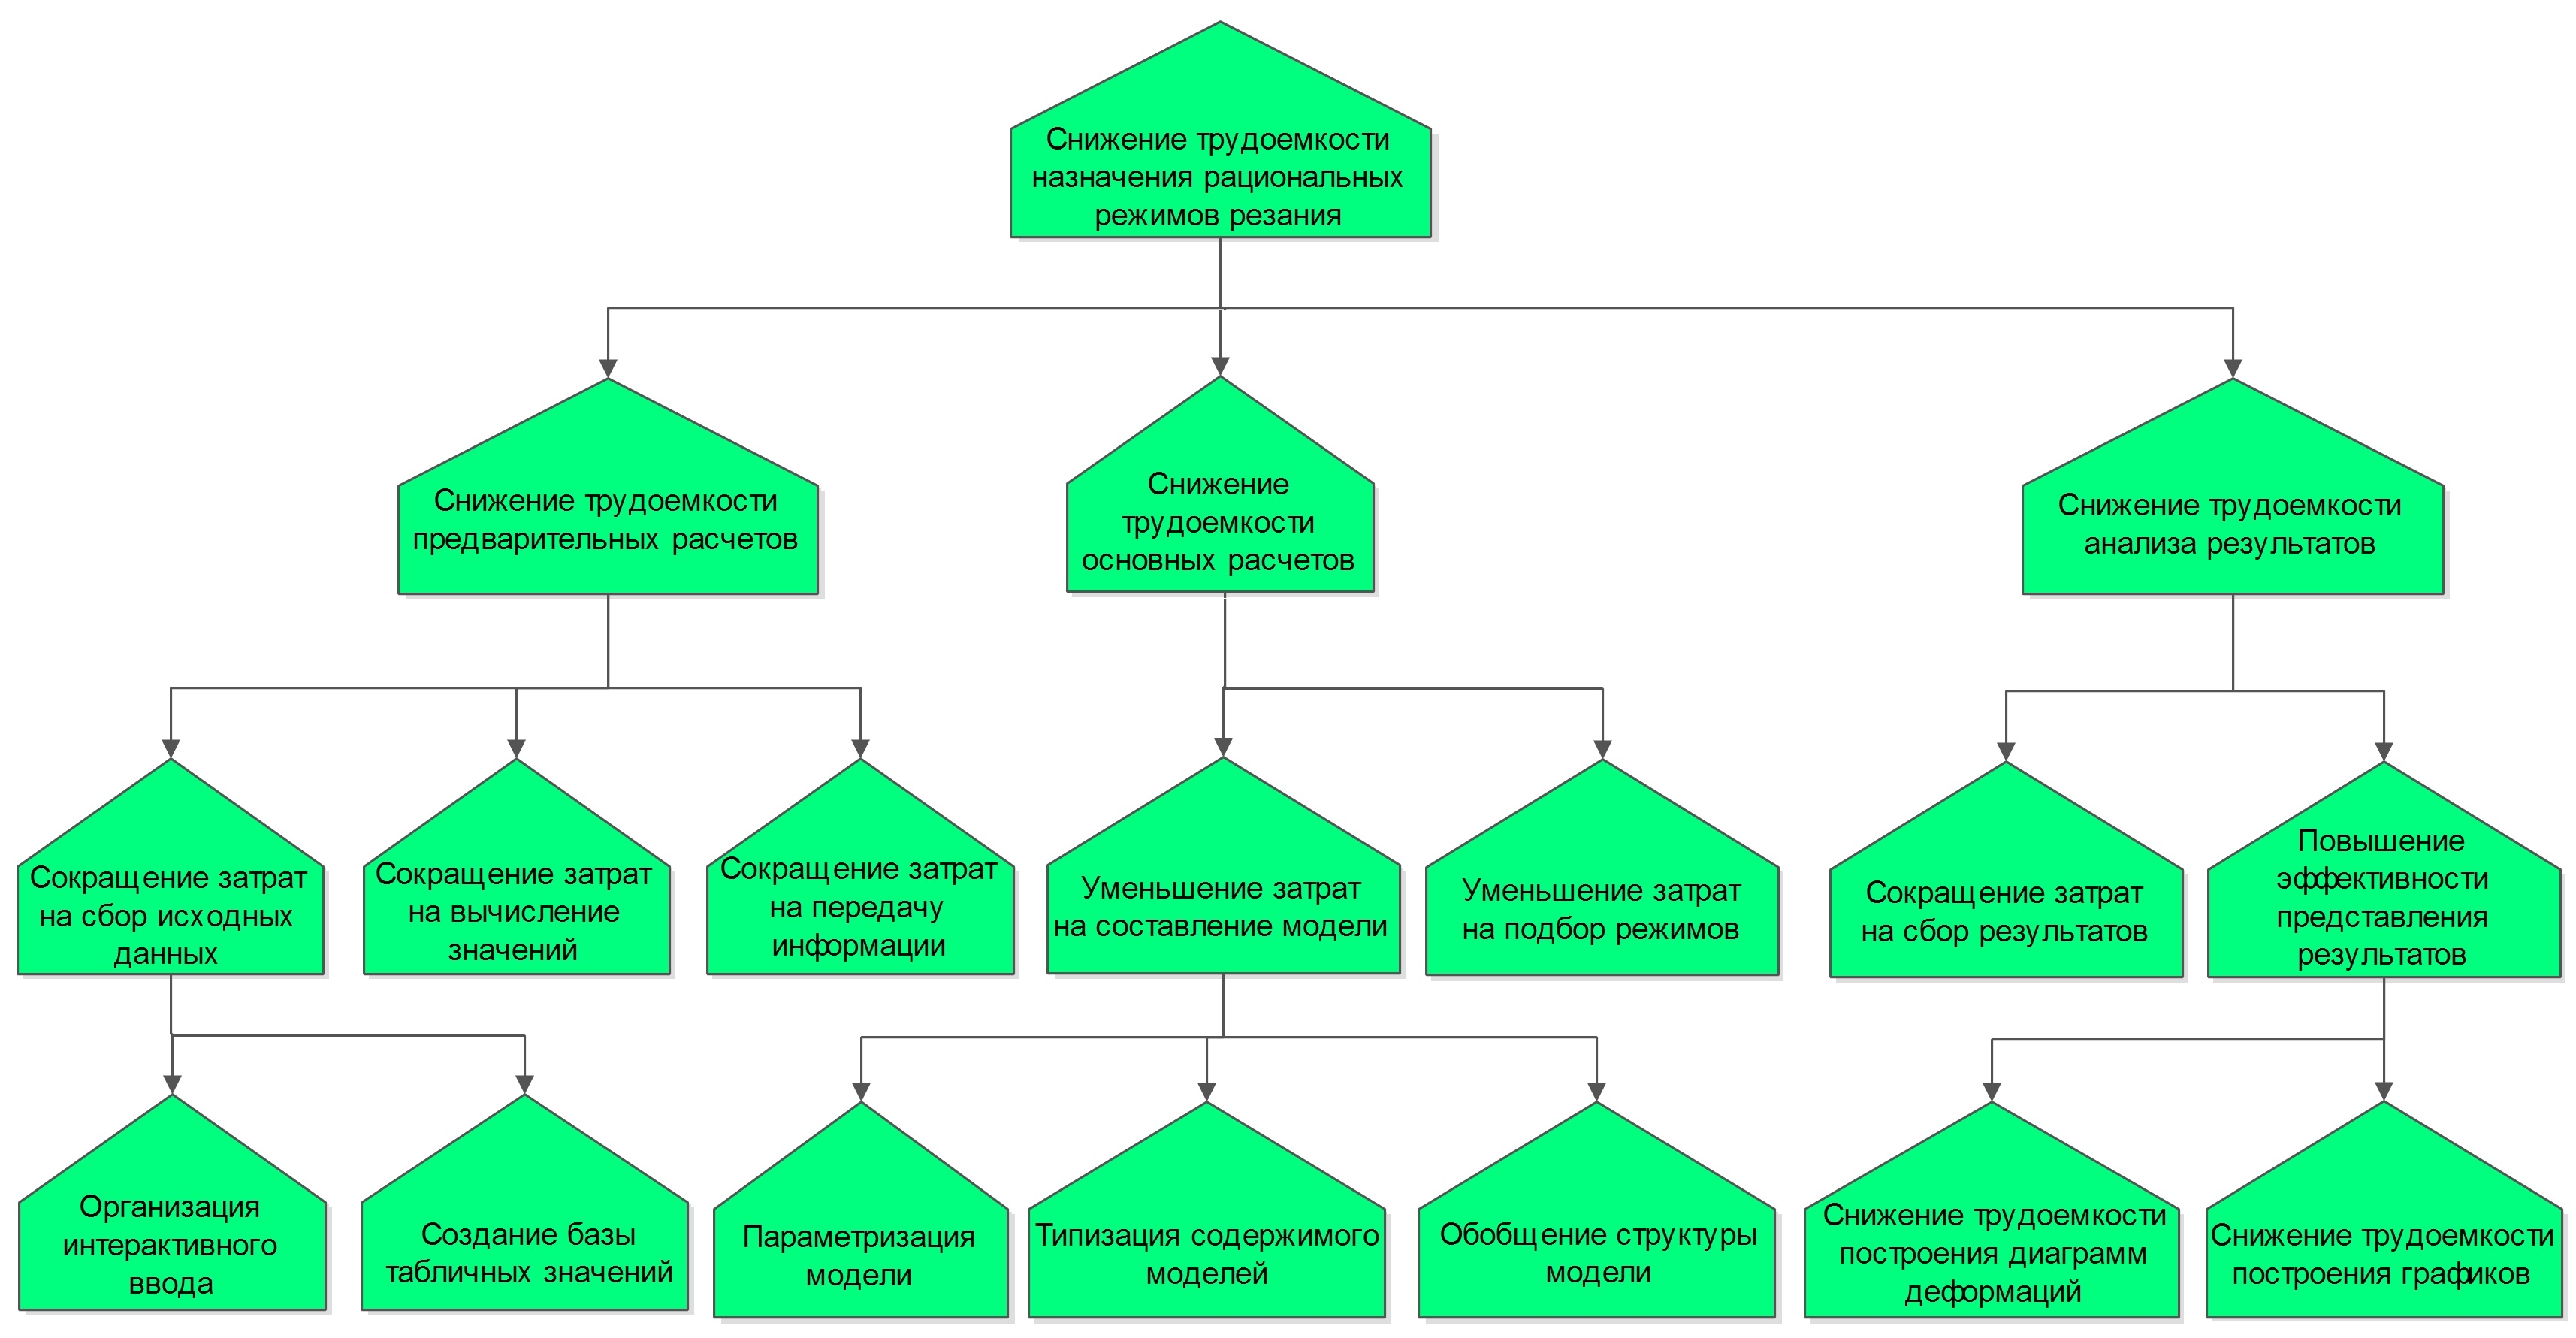
\includegraphics[scale=0.55]{img/at} 
	\end{center}
	\caption{Дерево целей}
	\label{fig:aim-tree}
	\end{figure}
	
	Снижение трудоемкости предварительных расчетов сводится к автоматизации вычисления режимов резания по традиционным методикам. Эта цель может быть достигнута при сокращении затрат на сбор исходных данных, вычисление значений и передачу информации. Под традиционными методиками понимается прежде всего таблично-аналитический подход, описанный в \cite{book:Kosilova}. Согласно указанной литературе, для вычисления параметров режима резания необходимо выбрать исходные данные из таблиц эмпирических коэффициентов и подставить их в приведенные в справочнике формулы. Снижение трудоемкости этих действий и образует первую подцель.
	
	Вторая задача состоит в том, чтобы разработать общую структуру модели, а также типизировать её содержимое. Путем параметризации может быть достигнуто эффективное повторное применение одной модели в рамках разработки различных технологических процессов. Используя внутренний расчетный механизм системы планируется обеспечить уменьшение затрат на подбор рациональных режимов резания. 
	
	После проведения расчетов требуется сделать вывод о допустимости принятых параметров обработки. Автоматизация построения диаграмм и графиков деформаций позволит повысить эффективность анализа результатов. 
	
	Дерево целей изображено на рисунке \ref{fig:aim-tree}. Оно систематизирует вышесказанное в виде иерархической структуры. 
		
	
				
	\section{Выбор языка программирования}
	Выбору языка программирования следует уделить особое внимание. От правильного решения существенно зависит насколько трудоемким будет процесс написания программы. Существующие языки программирования сильно различаются по возможностям, гибкости и области применения. На данном этапе необходимо рассмотреть основные варианты и выявить наилучший. 
	
	На стадии разработки концепции было выявлено, что следует опираться на подходы объектно-ориентированного программирования. Этот вывод соответствующим образом сужает область рассматриваемых решений. Для повышения пригодности продукта к обслуживанию также ограничимся общеизвестными и широко распространенными языками. Дополнительная выгода от использования таких языков состоит в возможности применения готовых компонентов и библиотек. 
	
	Под указанные ограничения подходят такие языки как С++, С\#, Java, Python. Сравним эти языки по существенным факторам методом непосредственной оценки. Для оценки будут приняты во внимание следующие характеристики: распространенность, скорость разработки, гибкость, безопасность. В рамках проекта производительность не рассматривается так как она не является ограничивающим фактором. По каждому критерию языку будет присвоен балл от 1 до 10. Наиболее предпочтительным будет признан язык с наибольшим суммарным баллом. 
	
	Распространенность может быть определена по числу проектов на информационном ресурсе github.com и числу заданных вопросов на stackoverflow.com. Эти ресурсы выбраны в качестве референтных из-за большой популярности в IT сообществе. Аналитическая фирма RedMonk опубликовала объективный рейтинг языков программирования в соответствии с указанными критериями \cite{web:RedMonk}. Этот отчет использован в качестве основания для присвоения баллов, поэтому Java получает максимальный балл, а остальные языки оценены меньшим числом. 
	
	Скорость разработки в большей мере субъективный параметр, так как он зависит не только от конструкций языка, но и от умений и опыта конкретного программиста, хотя можно выявить и общие тенденции. Скорость разработки рассматривается с учетом замечаний, изложенных в \cite{web:DZone}. Известно, что разработка на С++ требует больших временных затрат ввиду сложности конструкций и большого количества деталей, которые должны быть учтены программистом. По этому критерию предпочтение отдано Python, который относят к языкам сценариев. C\# и Java в плане скорости разработки не выделяются и получили средний балл.
	
	Гибкость также не поддается количественному определению, однако она зависит только от самого языка. Динамическая типизация позволила Python набрать максимальный балл. Также высоко оценены возможности ручного управления памятью в С++.
   
	\begin{table}[htb]
	\centering
	\caption{Оценка языков программирования}\label{tab:lang-rank} 
	\begin{tabularx}{\textwidth}{|l|Z|Z|Z|Z|}

		\hline Фактор & C++ & С\# & Java & Python \\ 
		\hline Распространенность & 9 & 9 & 10 & 9 \\ 
		\hline Скорость разработки & 8 & 9 & 9 & 10 \\ 
		\hline Гибкость & 10 & 9 & 9 & 10 \\ 
		\hline Безопасность & 8 & 10 & 10 & 8 \\ 
		\hline Итого & 36 & 37 & 38 & 37 \\ 
		\hline 
	\end{tabularx}
	\end{table}
	
	
	Безопасность в текущем контексте следует понимать как вероятность возникновения не обрабатываемых ошибок во время выполнения программы. Ошибки такого типа негативным образом сказываются на качестве программного продукта и наиболее затратны для исправления. Низкий балл Python обусловлен уже упомянутой особенностью  - динамической типизацией. В данном случае программист не имеет возможности воспользоваться описанием ошибок компиляции для устранения несоответствия типов переменных, это приводит к не обрабатываемым исключительным ситуациям уже во время выполнения. C++ также получил более низкую оценку ввиду общей сложности разработки и возможных ошибок при использовании адресной арифметики.
		
	Согласно таблице~\ref{tab:lang-rank} наиболее рациональным выбором является язык Java. Следует отметить, что оценка произведена с учетом требований к конкретному проекту и для других случаев на первый план могут выйти другие факторы.
	
	\section{Выбор модульной платформы}
	При описании модульной архитектуры в рамках концепции был оставлен открытым вопрос о средствах реализации. После выбора языка программирования можно вернуться к этому вопросу и проработать его более детально. 
	
	Многие эксперты в области программирования рекомендуют не разрабатывать сложные компоненты, если уже существуют достойные библиотеки, содержащие необходимый функционал \cite{Bloch}. В случае разработки на Java достичь модульной компоновки приложения можно при помощи одного из двух фреймворков: NetBeans Platform или Eclipse RCP. Детальный анализ показывает, что оба продукта в большей степени предоставляют эквивалентные возможности. Тем не менее были выделены следующие существенные различия: платформа NetBeans использует библиотеку Swing в качестве инструмента реализации пользовательского интерфейса, в то время как в Eclipse используется SWT. Немного более предпочтительным выглядит Swing, так как она является стандартной для Java и поставляется в комплекте разработчика (JDK - Java Development Kit) и поэтому имеет большое количество всевозможных сторонних расширений. Второе отличие в том, что в Eclipse модульная система реализована в соответствии со стандартом OSGi (Open Service Gateway Initiative) в то время как в NetBeans используется специфичная модульная система, хотя документация NetBeans также заявляет о частичной поддержке OSGi \cite{NetBeans}. В рамках проекта это отличие не представляется существенным. 
	
	В качестве программной платформы  было принято использовать NetBeans. На это решение повлияло наличие большого числа доступных ресурсов для освоения платформы, таких как проекты с открытым исходным кодом и обучающие официальные материалы а также подробная документация.

	\section{Выбор системы моделирования}
	Принцип моделирования подразумевает использование системы МКЭ расчетов при вычислении значений деформаций. Наиболее подходящими для этой цели были признаны ANSYS и SIMULA Abaqus FEA. Обе программы предоставляют богатый функционал, позволяющий моделировать рассматриваемый процесс обработки, поэтому функциональные критерии отходят на второй план. И ANSYS и Abaqus отвечают трем сформулированным ранее требованиям к системе моделирования. 
	
	Для выдачи расчетного задания в случае использования ANSYS имеется возможность организации взаимодействия через интерфейс командной строки. Модель может быть составлена на специальном предметно-ориентированным языке  ANSYS Parametric Design Language (APDL). Однако, анализ официальной документации не выявил ни одного  приемлемого способа передачи фактических значений параметров модели при вызове выполнения задания. Эта проблема может быть решена путем непосредственной замены значений в текстовом файле задания, но такой путь в большей степени подвержен вероятному возникновению ошибок, менее гибкий и более трудоемкий. Экспорт геометрии из ANSYS возможен только в единственном формате IGES. Хотя IGES широко используется в коммерческих CAD системах, для него не существует бесплатных Java библиотек визуализации, а реализация такой библиотеки (с учетом размера спецификации IGES около 700 страниц) не предоставляется возможной. 
	
	В плане возможностей интеграции с внешними системами выгодно отличается Abaqus. В Abaqus для описания модели используется язык общего назначения Python. При вызове расчетного задания через интерфейс командной строки есть возможность передачи значений параметров (например, геометрических размеров или силовых факторов). Также Abaqus поддерживает открытый формат OBJ для обмена геометрией. OBJ — это простой формат данных, для него существуют Java библиотеки, позволяющие отображать сохраненные модели. 
	
	Таким образом, для моделирования процесса будет использован Abaqus так как эта система более пригодна для взаимодействия с внешней информационной средой. 

	\chapter{Эскизное проектирование}
	\section{Определение функционала системы}
	На данном этапе необходимо определить какие функции должна выполнять разрабатываемая система. Для графического представления будет применена UML модель вариантов использования. Она описывает не только состав функций, но и их взаимосвязь с множеством действующих лиц. 
	
	Основная идея диаграммы вариантов использования состоит в отображении требований к системе через две базовые сущности - действующие лица и варианты использования. Пользователи и другие системы, которые могут взаимодействовать с продуктом называются действующими лицами, а вариант использования представляет собой спецификацию поведения \cite{spec:UML}. В системе предварительно можно выделить три лица, взаимодействующих с системой.
	
		\begin{figure}[!h]
		\begin{center}
		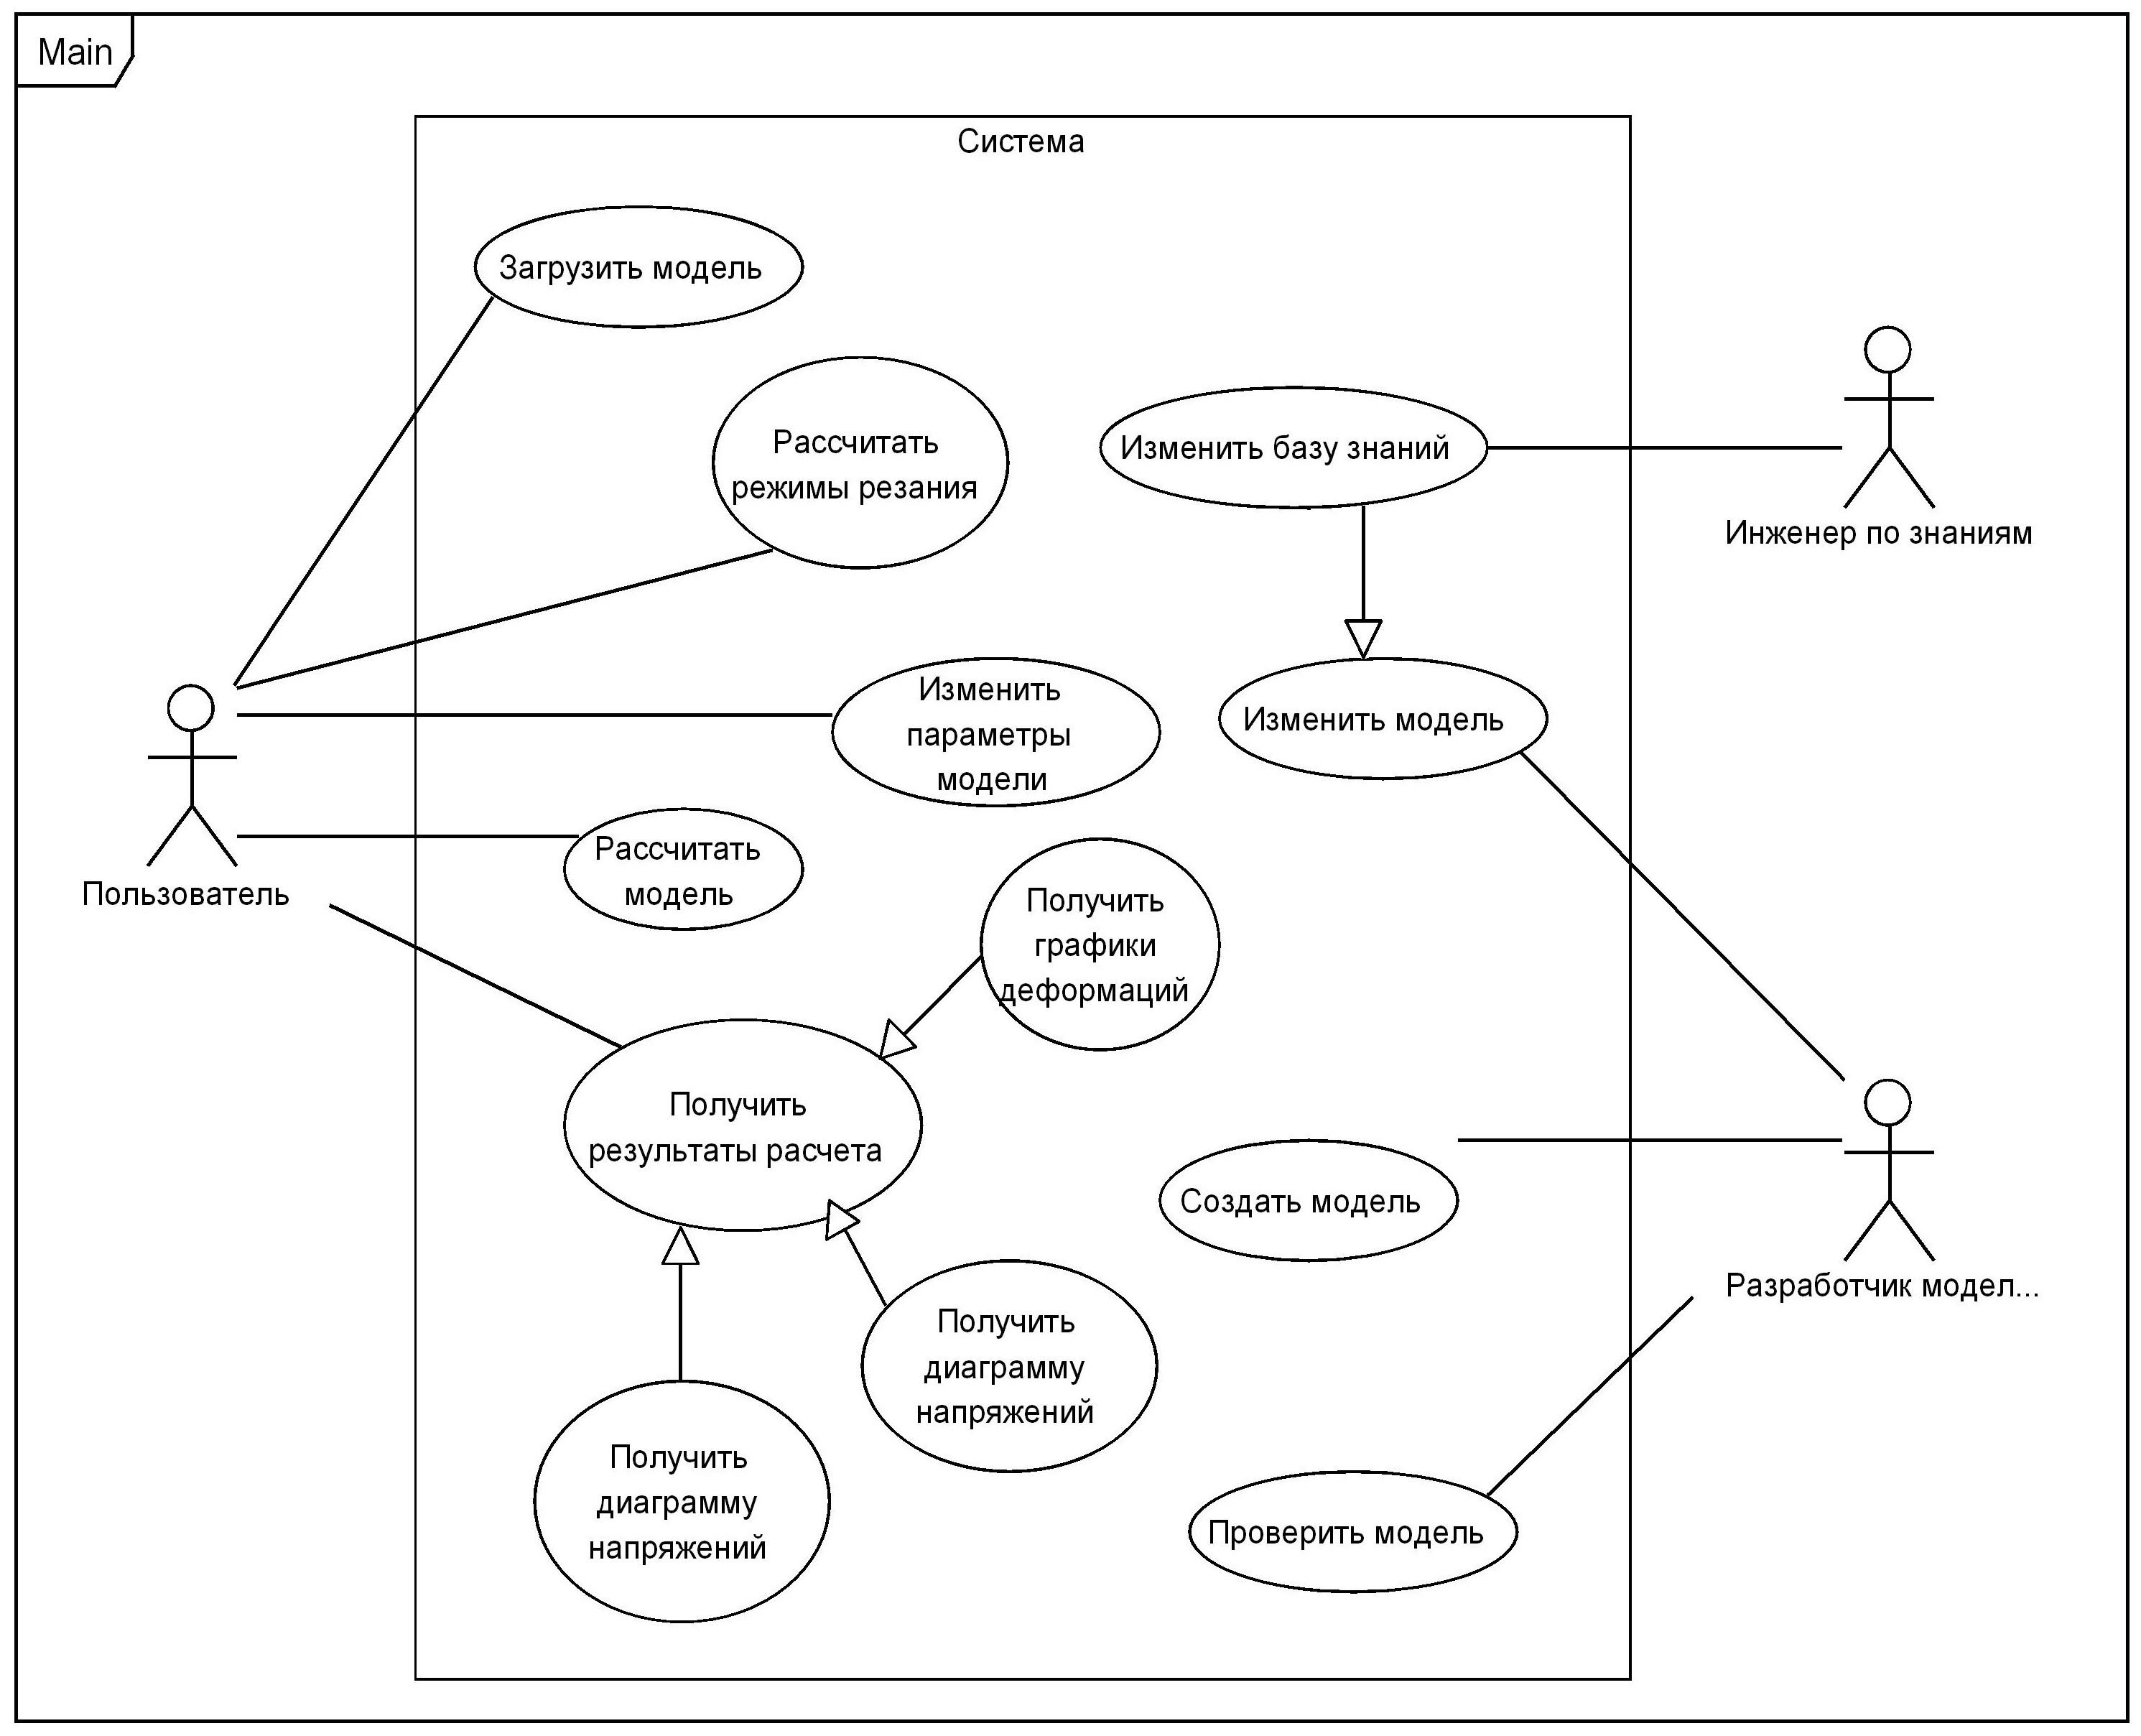
\includegraphics[scale=0.095]{img/ucd} 
		\end{center}
		\caption{Диаграмма вариантов использования}
		\label{fig:ucd}
		\end{figure}
		
	Первое лицо представленно пользователем, который заинтересован в выполнении функций, связанных с получением значений деформаций заготовки и их анализом. Для этого пользователю должна быть предоставлена возможность загрузки описания расчетного случая (то есть модели) в систему. Перед запуском расчета необходимо применить заданные характеристики процесса к параметризованной модели. По результатам работы CAE системы должны быть получены графики и диаграммы деформаций. Также пользователь ожидает от системы выполнения вспомогательных функций, таких как расчет режимов резания. 
	
	Необходимость выделения такого лица как инженер по знаниям обусловлена результатами анализа литературы \cite{book:Kosilova}, который показал, что для расчета режимов резания по таблично-аналитической методике потребуется представление экспертных знаний в формальном виде. Решение этой задачи возлагается на инженера по знаниям, который должен иметь возможность корректировать содержимое базы знаний.  

	Загружаемая в систему модель должна быть предварительно подготовлена компетентным экспертом --- разработчиком моделей. К обязанностям разработчика моделей относится также подготовка исходных данных в виде задания для выполнения CAE системой. После подготовки модели эксперт проверяет её работоспособность и при необходимости  устраняет дефекты, после чего предоставляет пользователю. 
	
	Составленная диаграмма вариантов использования изображена на рисунке \ref{fig:ucd}. Кроме описанных выше принципов на ней отображены зависимости обобщения между вариантами использования. Например, варианты использования ``Получить диаграмму деформаций'', ``Получить диаграмму напряжений'' и ``Получить графики деформаций'' обобщены в ``Получить результаты расчета''.  Указанная диаграмма будет использована для выделения отдельных элементов системы в модули для последующей проработке. 
	
	\chapter{Организационно-экономическая часть}
	\section{Введение}
	В данной главе рассматривается рассчет стоимости создания интегрированной системы поддержки принятия решения. 


	\section{Организация и планирование процесса разработки}
	Разработка интегрированной системы поддержки принятия решения является сложным процессом, стадии которого определяются при помощи ГОСТa Единой Системы Программной Документации \cite{gost:19102}. Согласно указанному документу всего выделяется 5 стадий, их подробное описание приведено в таблице \ref{tab:economy}. \textbf{{\MakeUppercase{Добавить таблицу}}}
	
	Основными факторами, определяющими трудоемкость создания интегрированной системы являются: степень новизны разрабатываемого программного комплекса, сложность алгоритма его функционирования, объем используемой информации, вид её представления и способ обработки, уровень языка программирования \cite{metoda:Economy}. Определим принадлежность разрабатываемого продукта к группам по каждому из указанных факторов. 
	
	По степени новизны интегрированная система может быть отнесена к группе <<Б>>: она не имеет аналогов, но и не требует разработки принципиально новых методов создания. 
	
	По степени сложности систему можно отнести к группе продукции, реализующей оптимизационные и моделирующие алгоритмы. Хотя непосредственная реализация метода конечных элементов не входит в рамки разработки продукта, тем не менее в составе системы имеется модуль управления моделированием. Принимая во внимание необходимость создания модели процесса обработки можно заключить что программа относится к группе 1. К тому же дальнейшее развитие проекта предполагает создание модуля многокритериальной оптимизации. 
	
	Как показал анализ литературы \cite{book:Kosilova}, исходная информация представлена как в виде формул, так и в виде разнородных таблиц. При этом требуется учитывать взаимное влияние данных, содержащихся в этих таблицах. Таким образом, разрабатываемую программу по виду представления исходной информации относят к группе 11. По структуре выходных документов система принадлежит группе 22 - требуется вывод на печать одинаковых документов, представляющих собой отчеты о моделировании.
	
	\section{Расчет трудоемкости этапов} 
	\subsection{Расчет трудоемкости разработки технического задания}
	Трудоемкость разработки технического задания может быть расчитана по формуле:
	\begin{equation}\label{eq:TZ}
		\tau_\textup{\scriptsize{ТЗ}} = T^{\textup{\scriptsize{З}}}_\textup{\scriptsize{РЗ}} + T^{\textup{\scriptsize{З}}}_\textup{\scriptsize{РП}},	
	\end{equation} 
	где	$\tau_\textup{\scriptsize{ТЗ}}$~--~трудоемкость разработки технического задания на создание программного продукта, \mbox{чел.-дни};\newline
	\phantom{где\space}$T^{\textup{\scriptsize{З}}}_\textup{\scriptsize{РЗ}}$~--~затраты времени разработчика постановки задачи на разработку ТЗ, \mbox{чел.-дни};\newline
	\phantom{где\space}$T^{\textup{\scriptsize{З}}}_\textup{\scriptsize{РП}}$~--~затраты времени разработчика программного обеспечения на разработку ТЗ, \mbox{чел.-дни}.\newline
	Значения величин $T^{\textup{\scriptsize{З}}}_\textup{\scriptsize{РЗ}}$ и $~ T^{\textup{\scriptsize{З}}}_\textup{\scriptsize{РП}}$ расчитывают по формулам: 
	\[
	T^{\textup{\scriptsize{З}}}_\textup{\scriptsize{РЗ}} = t_\textup{\scriptsize{З}} \cdot K^{\textup{\scriptsize{З}}}_\textup{\scriptsize{РЗ}}; \qquad	T^{\textup{\scriptsize{З}}}_\textup{\scriptsize{РП}} = t_\textup{\scriptsize{З}} \cdot K^{\textup{\scriptsize{З}}}_\textup{\scriptsize{РП}},
	\]
	где $ t_\textup{\scriptsize{З}}$~--~норма времени на разработку ТЗ на программный продукт, \mbox{чел.-дни}; $ t_\textup{\scriptsize{З}}=67$ \mbox{чел.-дни}, согласно таблице 2, приведенной в \cite{metoda:Economy} \newline
	\phantom{где\space}$K^{\textup{\scriptsize{З}}}_\textup{\scriptsize{РЗ}}$~--~коэффициент, учитывающий удельный вес трудоемкости работ, выполняемых разработчиком постановки задачи на стадии ТЗ; $K^{\textup{\scriptsize{З}}}_\textup{\scriptsize{РЗ}}=0,65$ для случая совместной с разработчиком ПО разработки.\newline
	\phantom{где\space}$K^{\textup{\scriptsize{З}}}_\textup{\scriptsize{РП}}$~--~коэффициент, учитывающий удельный вес трудоемкости работ, выполняемых разработчиком программного обеспечения на стадии ТЗ; $K^{\textup{\scriptsize{З}}}_\textup{\scriptsize{РП}}=0,35$ для совместной с разработчиком постановки задачи.\newline
	После подстановки принятых значений в (\ref{eq:TZ}) получаем:
	\[
	\tau_\textup{\scriptsize{ТЗ}} = 67 \cdot 0,65 + 67 \cdot 0,35 = 67 \enspace \mbox{чел.-дни}
	\]
	
	
	\subsection{Расчет трудоемкости выполнения эскизного проекта}
	Для расчета трудоемкости выполнения эскизного проекта (ЭП) используется формула:
	\begin{equation}\label{eq:EP}
	\tau_\textup{\scriptsize{ЭП}} = T^{\textup{\scriptsize{Э}}}_\textup{\scriptsize{РЗ}} + T^{\textup{\scriptsize{Э}}}_\textup{\scriptsize{РП}},	
	\end{equation} 
	где	$\tau_\textup{\scriptsize{ЭП}}$~--~трудоемкость разработки эскизного проекта, \mbox{чел.-дни};\newline
	\phantom{где\space}$T^{\textup{\scriptsize{Э}}}_\textup{\scriptsize{РЗ}}$~--~затраты времени разработчика постановки задачи на разработку ЭП, \mbox{чел.-дни};\newline
	\phantom{где\space}$T^{\textup{\scriptsize{Э}}}_\textup{\scriptsize{РП}}$~--~затраты времени разработчика программного обеспечения на разработку ЭП, \mbox{чел.-дни}.\newline
	Для расчета значений $T^{\textup{\scriptsize{Э}}}_\textup{\scriptsize{РЗ}}$ и $~ T^{\textup{\scriptsize{Э}}}_\textup{\scriptsize{РП}}$ могут быть применены следующие формулы:
	\[
	T^{\textup{\scriptsize{Э}}}_\textup{\scriptsize{РЗ}} = t_\textup{\scriptsize{Э}} \cdot K^{\textup{\scriptsize{Э}}}_\textup{\scriptsize{РЗ}}; \qquad	T^{\textup{\scriptsize{Э}}}_\textup{\scriptsize{РП}} = t_\textup{\scriptsize{Э}} \cdot K^{\textup{\scriptsize{Э}}}_\textup{\scriptsize{РП}},
	\]
	где $ t_\textup{\scriptsize{Э}}$~--~норма времени на разработку ЭП программного продукта, \mbox{чел.-дни}; $ t_\textup{\scriptsize{З}}=94$ \mbox{чел.-дни}, согласно таблице 3, приведенной в \cite{metoda:Economy} \newline
	\phantom{где\space}$K^{\textup{\scriptsize{Э}}}_\textup{\scriptsize{РЗ}}$~--~коэффициент, учитывающий удельный вес трудоемкости работ, выполняемых разработчиком постановки задачи на стадии ЭП; $K^{\textup{\scriptsize{Э}}}_\textup{\scriptsize{РЗ}}=0,7$ для случая совместной с разработчиком ПО разработки.\newline
	\phantom{где\space}$K^{\textup{\scriptsize{Э}}}_\textup{\scriptsize{РП}}$~--~коэффициент, учитывающий удельный вес трудоемкости работ, выполняемых разработчиком программного обеспечения на стадии ЭП; $K^{\textup{\scriptsize{Э}}}_\textup{\scriptsize{РП}}=0,3$ для совместной с разработчиком постановки задачи разработки ЭП.
	
	После подстановки принятых значений в (\ref{eq:EP}) получаем:
	\[
	\tau_\textup{\scriptsize{ТЗ}} = 94 \cdot 0,7 + 94 \cdot 0,3 = 94 \enspace \mbox{чел.-дни}
	\]
	
	
	\subsection{Расчет трудоемкости выполнения технического проекта}
	Трудоемкость разработки технического проекта $\tau_\textup{\scriptsize{ТП}}$ зависит от функционального назначения программного продукта, количества разновидностей форм входной и выходной информации и определяется по формуле:
	
	\begin{equation}\label{eq:TP}
	\tau_\textup{\scriptsize{ТП}} = (t^{\textup{\scriptsize{Т}}}_\textup{\scriptsize{РЗ}} + t^{\textup{\scriptsize{Т}}}_\textup{\scriptsize{РП}})  K_{\textup{\scriptsize{В}}} \cdot K_{\textup{\scriptsize{Р}}}
	\end{equation} 
	где $t^{\textup{\scriptsize{Т}}}_\textup{\scriptsize{РЗ}}, 
	\enspace t^{\textup{\scriptsize{Т}}}_\textup{\scriptsize{РП}}$~--~норма времени, затрачиваемого на разработку ТП разработчиком постановки задач и разработчиком программного обеспечения соответственно, \mbox{чел.-дни}; по таблице 16 в \cite{metoda:Economy} определено, что для принятой группы сложности алгоритма и степени новизны программной продукции нормы времени составляют $t^{\textup{\scriptsize{Т}}}_\textup{\scriptsize{РЗ}}=89 \enspace \mbox{чел.-дни}$ и  $t^{\textup{\scriptsize{Т}}}_\textup{\scriptsize{РП}}=64 \enspace \mbox{чел.-дни}$ 
	\newline
	\phantom{где\space}$K_\textup{\scriptsize{В}}$~--~коэффициент учета вида используемой информации;\newline
	\phantom{где\space}$K_\textup{\scriptsize{Р}}$~--~коэффициент учета режима обработки информации; по таблице 17 приведенной в \cite{metoda:Economy} определено значение $K_\textup{\scriptsize{Р}} = 1,45$.\newline
	Значение коэффициента $K_\textup{\scriptsize{В}}$ определяют из выражения:
	\begin{equation}\label{eq:KV}
	K_\textup{\scriptsize{В}} = \frac{K_\textup{\scriptsize{П}} \cdot n_\textup{\scriptsize{П}} + K_\textup{\scriptsize{НС}} \cdot n_\textup{\scriptsize{НС}}+ K_\textup{\scriptsize{Б}} \cdot n_\textup{\scriptsize{Б}}}{n_\textup{\scriptsize{П}} + n_\textup{\scriptsize{НС}} + n_\textup{\scriptsize{Б}}}
	\end{equation} 
	где $ K_\textup{\scriptsize{П}}$, $ K_\textup{\scriptsize{НС}} $,  $ K_\textup{\scriptsize{Б}}$~--~значения коэффициентов учета вида информации для переменной, нормативно-справочной информации и баз данных соответственно. Согласно таблице 18 методических указаний \cite{metoda:Economy} для группы новизны <<Б>>:	$ K_\textup{\scriptsize{П}} = 1,20; \enspace K_\textup{\scriptsize{НС}} = 1,08; \enspace K_\textup{\scriptsize{Б}} =3,12	$. \newline
	\phantom{где\space} $n_\textup{\scriptsize{П}}$, $n_\textup{\scriptsize{НС}}$, $n_\textup{\scriptsize{Б}}$~--~количество наборов данных переменной, нормативно-справочной информации и баз данных соответственно. Для разрабатываемой интегрированной системы $n_\textup{\scriptsize{П}}=2; \enspace n_\textup{\scriptsize{НС}}=1; \enspace n_\textup{\scriptsize{Б}}=0$.  

	После подстановки определенных значений коэффициентов учета вида информации и количества наборов данных в формулу (\ref{eq:KV}) получаем:
	\[
		K_\textup{\scriptsize{В}} = \frac{1,20 \cdot 2 + 1,08 \cdot 1+ 3,12 \cdot 0	} {2 + 1 + 0} = 1,16
	\]
	Для рассчитанного значения $K_\textup{\scriptsize{В}}$ по формуле (\ref{eq:TP}) получаем значение трудоемкости выполнения технического проекта:
	\[
		\tau_\textup{\scriptsize{ТП}} = (89 + 64) \cdot 1,16 \cdot 1,45 = 257 \enspace \mbox{чел.-дни}
	\]
	
	\subsection{Расчет трудоемкости выполнения рабочего проекта}
	Трудоемкость разработки рабочего проекта зависит от функционального назначения программного продукта, количества разновидностей форм входной и выходной информации, сложности алгоритма функционирования, степени использования готовых программных модулей и уровня алгоритмического языка программирования и определяется по формуле:
 	\begin{equation}\label{eq:TRP}
 			\tau_\textup{\scriptsize{РП}} = K_\textup{\scriptsize{К}} \cdot K_\textup{\scriptsize{Р}} \cdot K_\textup{\scriptsize{Я}} \cdot K_\textup{\scriptsize{З}} \cdot K_\textup{\scriptsize{ИА}}  (t^{\textup{\scriptsize{Р}}}_\textup{\scriptsize{РЗ}} + t^{\textup{\scriptsize{Р}}}_\textup{\scriptsize{РП}})
 	\end{equation}
 	где $K_\textup{\scriptsize{К}} $~--~коэффициент учета сложности контроля информации; $K_\textup{\scriptsize{К}}=1,07$ в соответствии с таблицей 19 методических указаний \cite{metoda:Economy}.\newline
 	\phantom{где\space}$K_\textup{\scriptsize{Р}}$~--~коэффициент учета режима обработки информации; ранее определено что $K_\textup{\scriptsize{Р}} = 1,45$. \newline
 	\phantom{где\space}$K_\textup{\scriptsize{Я}} $~--~коэффициент учета уровня используемого языка программирования; $K_\textup{\scriptsize{Я}} = 1 $ для языка высокого уровня.\newline
 	\phantom{где\space}$K_\textup{\scriptsize{З}} $~--~коэффициент учета степени использования готовых программных модулей; с учетом применения готового расчетного ядра МКЭ моделирования и большого количества стандартных библиотек $K_\textup{\scriptsize{З}} =0,6$. \newline
 	\phantom{где\space}$K_\textup{\scriptsize{ИА}} $~--~коэффициент учета вида используемой информации и сложности алгоритма;\newline
 	Значение $K_\textup{\scriptsize{ИА}} $ вычисляется по формуле:
 	\begin{equation}\label{eq:KIA}
 	 	K_\textup{\scriptsize{ИА}} = \frac{	K^\prime_\textup{\scriptsize{П}} n_\textup{\scriptsize{П}} + 	K^\prime_\textup{\scriptsize{НС}} n_\textup{\scriptsize{НС}} +	K^\prime_\textup{\scriptsize{Б}} n_\textup{\scriptsize{Б}} }{n_\textup{\scriptsize{П}} + n_\textup{\scriptsize{НС}} + n_\textup{\scriptsize{Б}}}
 	\end{equation}
 	где $K^\prime_\textup{\scriptsize{П}}$, $K^\prime_\textup{\scriptsize{НС}}$, $	K^\prime_\textup{\scriptsize{Б}}$~--~значения коэффициентов учета сложности алгоритма программного продукта и вида используемой информации для переменной, нормативно-справочной информации и баз данных соответственно; согласно таблице 22 методических указаний \cite{metoda:Economy} для группы новизны <<Б>> и группы 1 сложности алгоритма $K^\prime_\textup{\scriptsize{П}}=1,62$, $K^\prime_\textup{\scriptsize{НС}}=0,97$, $	K^\prime_\textup{\scriptsize{Б}}=0,81$. \newline
	\phantom{где\space}$t^{\textup{\scriptsize{Р}}}_\textup{\scriptsize{РЗ}}$, $t^{\textup{\scriptsize{Р}}}_\textup{\scriptsize{РП}}$~--~норма времени затраченного на разработку программы на языке высокого уровня разработчиком постановки задач и разработчиком программного обеспечения соответственно, чел.-дни; ранее определено что трудоемкость выполнения технического проекта для разработчика постановки задач	$t^{\textup{\scriptsize{Т}}}_\textup{\scriptsize{РЗ}} =  89 \enspace \mbox{чел.-дни}$, тогда по таблице 35а $t^{\textup{\scriptsize{Р}}}_\textup{\scriptsize{РЗ}}=107 \enspace \mbox{чел.-дни}$, а трудоемкость выполнения технического проекта разработчиком программного обеспечения $t^{\textup{\scriptsize{Т}}}_\textup{\scriptsize{РП}} = 64 \enspace \mbox{чел.-дни}$, следовательно $t^{\textup{\scriptsize{Р}}}_\textup{\scriptsize{РП}}=683 \enspace \mbox{чел.-дни}$.
	Подставим табличные значения в формулу (\ref{eq:KIA}):
 	\[
 	 	 	K_\textup{\scriptsize{ИА}} = \frac{1,62 \cdot 2 + 0,97 \cdot 1 +	0,81 \cdot 0 }{2+1+0}=1,40
 	 \]
 	 Тогда трудоемкость разработки рабочего проекта по формуле (\ref{eq:TRP}):
 	 \[
 	  			\tau_\textup{\scriptsize{РП}} = 1,07 \cdot 1,45 \cdot 1 \cdot 0,6 \cdot 1,40 (107 + 683)=735  \enspace \mbox{чел.-дни}
 	  \]
 	  
	\subsection{Расчет трудоемкости стадии внедрения}
	Трудоемкость выполнения стадии ``Внедрение'' $\tau_\textup{\scriptsize{В}}$ может быть расчитана по формуле 
	\begin{equation}\label{eq:TV}
	\tau_\textup{\scriptsize{В}} = (t^{\textup{\scriptsize{В}}}_\textup{\scriptsize{РЗ}} + t^{\textup{\scriptsize{В}}}_\textup{\scriptsize{РП}}) K_\textup{\scriptsize{К}} \cdot K_\textup{\scriptsize{Р}}  \cdot K_\textup{\scriptsize{З}} 
	\end{equation}
	где $t^{\textup{\scriptsize{В}}}_\textup{\scriptsize{РЗ}}$, $t^{\textup{\scriptsize{В}}}_\textup{\scriptsize{РП}}$~--~норма времени, затрачиваемого разработчиком постановки задачи и разработчиком программного обеспечения соответственно на выполнение процедур внедрения, чел.-дни; исходя из таблицы 48 \mbox{$t^{\textup{\scriptsize{В}}}_\textup{\scriptsize{РЗ}}=33 \enspace  \mbox{чел.-дни}$}, $t^{\textup{\scriptsize{В}}}_\textup{\scriptsize{РП}}=98 \enspace  \mbox{чел.-дни}$. \newline
	При подстановке норм времени и коэффициентов учета в формулу (\ref{eq:TV}) получаем:
	\[
		\tau_\textup{\scriptsize{В}} = (33 + 98) 1,07 \cdot 1,45  \cdot 0,6 = 122 \enspace  \mbox{чел.-дни}
	\]

	\subsection{Расчет суммарной трудоемкости и продолжительности работ}
	Полученные на предыдущих этапах результаты могут быть сведены в таблицу \ref{tab:economyTrud}. Общая трудоемкость разработки программной продукции равна сумме величин трудоемкости выполнения отдельных стадий: $\tau_\textup{\scriptsize{ПП}} = \tau_\textup{\scriptsize{ТЗ}} +\\+ \tau_\textup{\scriptsize{ЭП}} + \tau_\textup{\scriptsize{ТП}} + \tau_\textup{\scriptsize{РП}} + \tau_\textup{\scriptsize{В}} = 67 + 94 +257 + 735 + 122 = 1293 \enspace \mbox{чел.-дни}$. 
	
	Для целей планирования и контроля используют ленточный график исходя из того что разработку осуществляет небольшой, стабильный по составу коллектив исполнителей. 
	\begin{table}[htb]
		\centering
		\caption{Трудоемкости стадий}\label{tab:economyTrud} 
		\begin{tabularx}{\textwidth}{|l|Z|Z|Z|}
			\hline Стадия разработки & Трудоемкость, \mbox{чел.-дни} & Число исполнителей & Зарплата исполн., руб \\ 
			\hline Техническое задание & 67 & 1 & 40 000\\ 
			\hline Эскизный проект & 94 & 2 &  42 000\\ 
			\hline Технический проект & 257 & 3 & 40 000 \\ 			
			\hline Рабочий проект & 735 & 3 & 40 000\\ 			
			\hline Внедрение & 122 & 2 & 38 000\\ 
			\hline 
		\end{tabularx}
	\end{table}
	Продолжительность выполнения всех работ по этапам разработки определяют из выражения:
	\begin{equation}\label{eq:TI}
	T_\textup{\scriptsize{i}} = \frac{\tau_\textup{\scriptsize{i}} + Q}{n_\textup{\scriptsize{i}}}
	\end{equation}
	где $\tau_\textup{\scriptsize{i}}$~--~трудоемкость $i\mbox{-й}$ работы, \mbox{чел.-дни};\newline
	\phantom{где\space}$Q$~--~трудоемкость дополнительных работ, выполняемых исполнителем, \mbox{чел.-дни};\newline
	\phantom{где\space}$n_\textup{\scriptsize{i}}$~--~количество исполнителей, выполняющих  $i\mbox{-ю}$ работу, чел.\newline
	Для разрабатываемой интегрированной системы назначим одного исполнителя для подготовки технического задания, двух -- для работ по внедрению продукта и выполнения эскизного проекта и трех исполнителей для разработки технического и рабочего проектов.  Тогда по формуле (\ref{eq:TI}) продолжительность разработки программного продукта:
	\jot = 15pt
	 \begin{eqnarray}
		\begin{aligned}
			& T_\textup{\scriptsize{ТЗ}} = \frac{67}{1} = 67 \enspace \mbox{дни};   & T_\textup{\scriptsize{ЭП}} = \frac{94}{2} = 47 \enspace \mbox{дни}; & \quad 	 T_\textup{\scriptsize{ТП}} = \frac{257}{3} = 86 \enspace \mbox{дни}; \nonumber \\ & T_\textup{\scriptsize{РП}} = \frac{735}{3} = 245 \enspace \mbox{дни};  & T_\textup{\scriptsize{В}} = \frac{122}{2} = 61 \enspace \mbox{дни}; & \quad T_{\scriptsize{\Sigma}} = 506 \enspace \mbox{дни};\nonumber
		\end{aligned} 
	\end{eqnarray}

	
	\section{Определение затрат на разработку программной продукции} 
	Затраты на разработку программной продукции могут быть представлены в виде суммы основных статей расходов, таких как материалы, специальное оборудование, основная заработная плата, дополнительная заработная плата, отчисления на социальное страхование, накладные расходы.
	\subsection{Расчет основной заработной платы}
	В основную заработную плату включается заработная плата всех исполнителей, непосредственно занятых разработкой программного продукта, с учетом их должностного оклада и времени участия в разработке. Расчет ведется по формуле:
	\begin{equation}\label{eq:ZO}
		C_\textup{\scriptsize{ЗО}} = \sum_{i}^{}\frac{\textup{З}_{\scriptsize{i}}}{d}\tau_{\scriptsize{i}}
	\end{equation}
	где $\textup{З}_{\scriptsize{i}}$~--~среднемесячный оклад $i\mbox{-го}$ исполнителя, руб.\newline
	\phantom{где\space}$d$~--~среднее количество рабочих дней в месяце;\newline
	\phantom{где\space}$\tau_{\scriptsize{i}}$~--~трудоемкость работ, выполняемых $i\mbox{-м}$ исполнителем, чел.-дни.
	\[
			C_\textup{\scriptsize{ЗО}} = \frac{40000}{21} \cdot 67 + \frac{42000}{21} \cdot 94 +  \frac{40000}{21} \cdot 257 + \frac{40000}{21} \cdot 735 + \frac{38000}{21} \cdot 122 = 2311048\enspace\mbox{руб.}
	\]
	\subsection{Расчет дополнительной заработной платы}
	Дополнительная заработная плата учитывает все выплаты непосредственным исполнителям за время (установленное законодательством), непроработанное на производстве, в том числе: оплата очередных отпусков, компенсауия за неиспользованный отпуск и др. Расчет ведется по формуле:
	\[
		C_\textup{\scriptsize{ЗД}} = C_\textup{\scriptsize{ЗО}} \cdot \alpha_\textup{\scriptsize{Д}}
	\]
	где $\alpha_\textup{\scriptsize{Д}}$~--~коэффициент отчислений на дополнительную зарплату $\alpha_\textup{\scriptsize{Д}}=0,2$.
	\[
		C_\textup{\scriptsize{ЗД}} =  2311048 \cdot 0,2 = 462210\enspace\mbox{руб.}
	\]
	\subsection{Отчисления на социальное страхование}
	В статье учитываются отчисления в бюджет социального страхования по установленному законодательством тарифу от суммы основной и дополнительной заработной платы:
	\[
	C_\textup{\scriptsize{СС}} =  \alpha_\textup{\scriptsize{СС}} \cdot (	C_\textup{\scriptsize{ЗО}} + 	C_\textup{\scriptsize{ЗД}})
	\]
	где $\alpha_\textup{\scriptsize{СС}}$~--~коэффициент отчислений на социальное страхование; $\alpha_\textup{\scriptsize{СС}} = 0,3 +\\+ 0,002 = 0,302$.
	\[
	C_\textup{\scriptsize{СС}} =  0,302 \cdot (2311048+462210) = 263724\enspace\mbox{руб.}
	\]
	\subsection{Накладные расходы}
	В статье учитываются затраты на общехозяйственные расходы, непроизвольные расходы и расходы на управление. Накладные расходы определяют в процентном отношении к основной заработной плате:
	\[
		C_\textup{\scriptsize{Н}} =  \alpha_\textup{\scriptsize{Н}} \cdot 	C_\textup{\scriptsize{ЗО}}
	\]
	где $\alpha_\textup{\scriptsize{Н}}$~--~коэффициент накладных расходов;  $\alpha_\textup{\scriptsize{Н}}=1,8$.
	\[
	C_\textup{\scriptsize{Н}} =  1,8 \cdot 2311048 = 4159886\enspace\mbox{руб.}
	\]
	\subsection{Расходы на оборудование}
	В статье учитываются суммарные затраты на приобретение или проектирование необходимого оборудования. Таблица \ref{tab:economySpecOb} отображает предполагаемое количество и цену используемого оборудования. 
	\begin{table}[htb]
		\centering
		\caption{Специальное оборудование}\label{tab:economySpecOb} 
		\begin{tabularx}{\textwidth}{|l|Z|Z|l|Z|Z|}
			\hline \No & Наименование & Единица измерения & Кол-во & Цена за единицу, руб. & Сумма, руб.\\ 
			\hline 1 & ПЭВМ & шт & \multicolumn{1}{|c|}{9} & 40000 & 360000\\
			\hline 
		\end{tabularx}
	\end{table}
	 
	 В случае использования оборудования для разработки нескольких программных продуктов, его стоимость распределяется между всеми продуктами пропорционально времени использования:
	\[
	C_\textup{\scriptsize{СО}} = \sum_{i}^{} \frac{  C_{\textup{\scriptsize{Б}}i} \cdot \alpha_i }{100 F_\textup{\scriptsize{Д}}}t_i
	\]
	где $ C_{\textup{\scriptsize{Б}}i}$~--~балансовая цена $i\mbox{-го}$ вида оборудования, руб.;\newline
	\phantom{где\space}$\alpha_i$~--~норма годовых амортизационных отчислений для оборудования $i\mbox{-го}$ вида, \%; $\alpha_i=12,0\enspace\mbox{\%}$ по таблице 50 методических указаний \cite{metoda:Economy};\newline
	\phantom{где\space}$F_\textup{\scriptsize{Д}}$~--~действительный годовой фонд времени, ч; $F_\textup{\scriptsize{Д}} = 2080 \enspace \mbox{ч}$ при 8-ми часовом рабочем дне и 5-ти дневной рабочей недели;\newline
	\phantom{где\space}$t_i$~--~время использования $i\mbox{-го}$ вида оборудования для выполнения данной разработки, ч.
	Затраты на оборудование:
	\[
			C_\textup{\scriptsize{СО}} = \frac{ 40000 \cdot 12 }{100 \cdot 2080} \enspace 506 \cdot 8 =9341 \mbox{руб.}
	\]
	
	\subsection{Результаты расчета затрат}
	По итогам расчетов затрат на разработку программной продукции составлена обобщающая таблица \ref{tab:economyResult}:
	\begin{table}[htb]
			\centering
			\caption{Результаты расчета затрат}\label{tab:economyResult} 
			\begin{tabularx}{\textwidth}{|l|l|Z|}
				\hline \No & Наименование & Сметная стоимость, руб.\\ 
				\hline 1 & Основная заработная плата & 2 311 048\\
				\hline 2 & Дополнительная заработная плата & 462 210\\
				\hline 3 & Отчисления на социальное страхование & 263 724\\
				\hline 4 & Накладные расходы & 4 159 886\\
				\hline 5 & Расходы на использование оборудования & 9 341\\				
				\hline  & Итого & 7 206 209\\								
				\hline 
			\end{tabularx}
	\end{table}
	\section{Выводы}		
		\begin{itemize}
			\item Суммарная трудоемкость разработки программного продукта составляет 1293 чел.-дней.
			\item Продолжительность выполнения работ всех стадий с учетом принятого числа исполнителей составляет 506 раб. дней.
			\item Общие расходы на разработку программного продукта составляют \mbox{7 206 209 руб.}
		\end{itemize}
 %\begin{enumerate}
%		\item Эскизный проект
%		\item Технический проект
%		\item Рабочий проект
%		\item Внедрение
%	\end{enumerate}
	
%	\begin{table}[htb]
%		\centering
%		\caption{Стадии разработки}\label{tab:economy} 
%		\begin{tabularx}{\textwidth}{|l|X|}
%			
%			\hline Стадия разработки & \multicolumn{1}{|Z|}{Состав выполняемых работ }\\ 
%			\hline Техническое задание & Постановка задач, определение функционального и эксплуатационного назначения, требований к продукту, сбор исходных материалов  \\ 
%			\hline Эскизный проект &  \\ 
%			\hline Технический проект &  \\ 			
%			\hline Рабочий проект &  \\ 			
%			\hline Внедрение &  \\ 
%			\hline 
%		\end{tabularx}
%	\end{table}
	
	\renewcommand{\bibname}{\centerline{\large{Список литературы}}}
	\bibliographystyle{utf8gost705u} 

	\bibliography{biblio}
	\addcontentsline{toc}{chapter}{Список литературы} % добавляем пункт "Литература" в
	%\nocite{Exp1}
	%\nocite{OOP}
	%\nocite{Java1}
	%\nocite{Java2}
	%\nocite{Exp2}
	
	
%	\chapter{Предпроектное исследование}
%	
%		\section{Введение}
%		Д
%
%		 \begin{figure}[!h]
%		 \begin{center}
%		 \includegraphics[scale=0.07]{img/ProjectHistory} 
%		 \end{center}
%		 \caption{История развития работ}
%		 \label{ris:ProjectHistory}
%		 \end{figure}
%		
%	
%	\section{Выбор программных средств}
%		\subsection{Выбор системы моделирования}
	
\end{document}